\documentclass{article}
\usepackage[utf8]{inputenc}
\usepackage{polski}
\usepackage[polish]{babel}
\usepackage{bbm}
\usepackage{amsmath}
\usepackage{amsthm}
\usepackage{graphicx}
\usepackage{epstopdf}
\usepackage[export]{adjustbox}
\usepackage{float}
\usepackage{listings}

\newtheorem{defi}{Definicja}
\newtheorem{twr}{Twierdzenie}
\newtheorem*{dd}{Dowód}

\DeclareMathOperator{\sign}{sign}
\DeclareMathOperator{\arctg}{arctg}

\newcommand{\twopartdef}[4]
{
	\left\{
		\begin{array}{ll}
			#1 & \mbox{jeśli } #2 \\
			#3 & \mbox{jeśli } #4
		\end{array}
	\right.
}


\author{Jarosław Dzikowski 273233}
\date{Wrocław, \today}
\title{\textbf{Bazy danych} \\ Rowery miejskie - dokumentacja}
\begin{document}
\maketitle

\section{Zawartość dokumentacji}
Dokument składa się z trzech części:
\begin{enumerate}
	\item Tej części ostatecznego modelu konceptualnego, która została zaimplementowana w aplikacji.
	\item Instrukcja instalacji aplikacji.
	\item Dokumentacja aplikacji.
\end{enumerate}

\section{Ostateczny model konceptualny}
Diagram E-R został zamieszczony na osobnej stronie ze względu na swoją wielkość.
\pagenumbering{gobble}% Remove page numbers (and reset to 1)
%\clearpage
\begin{figure}[p]
\centerline{	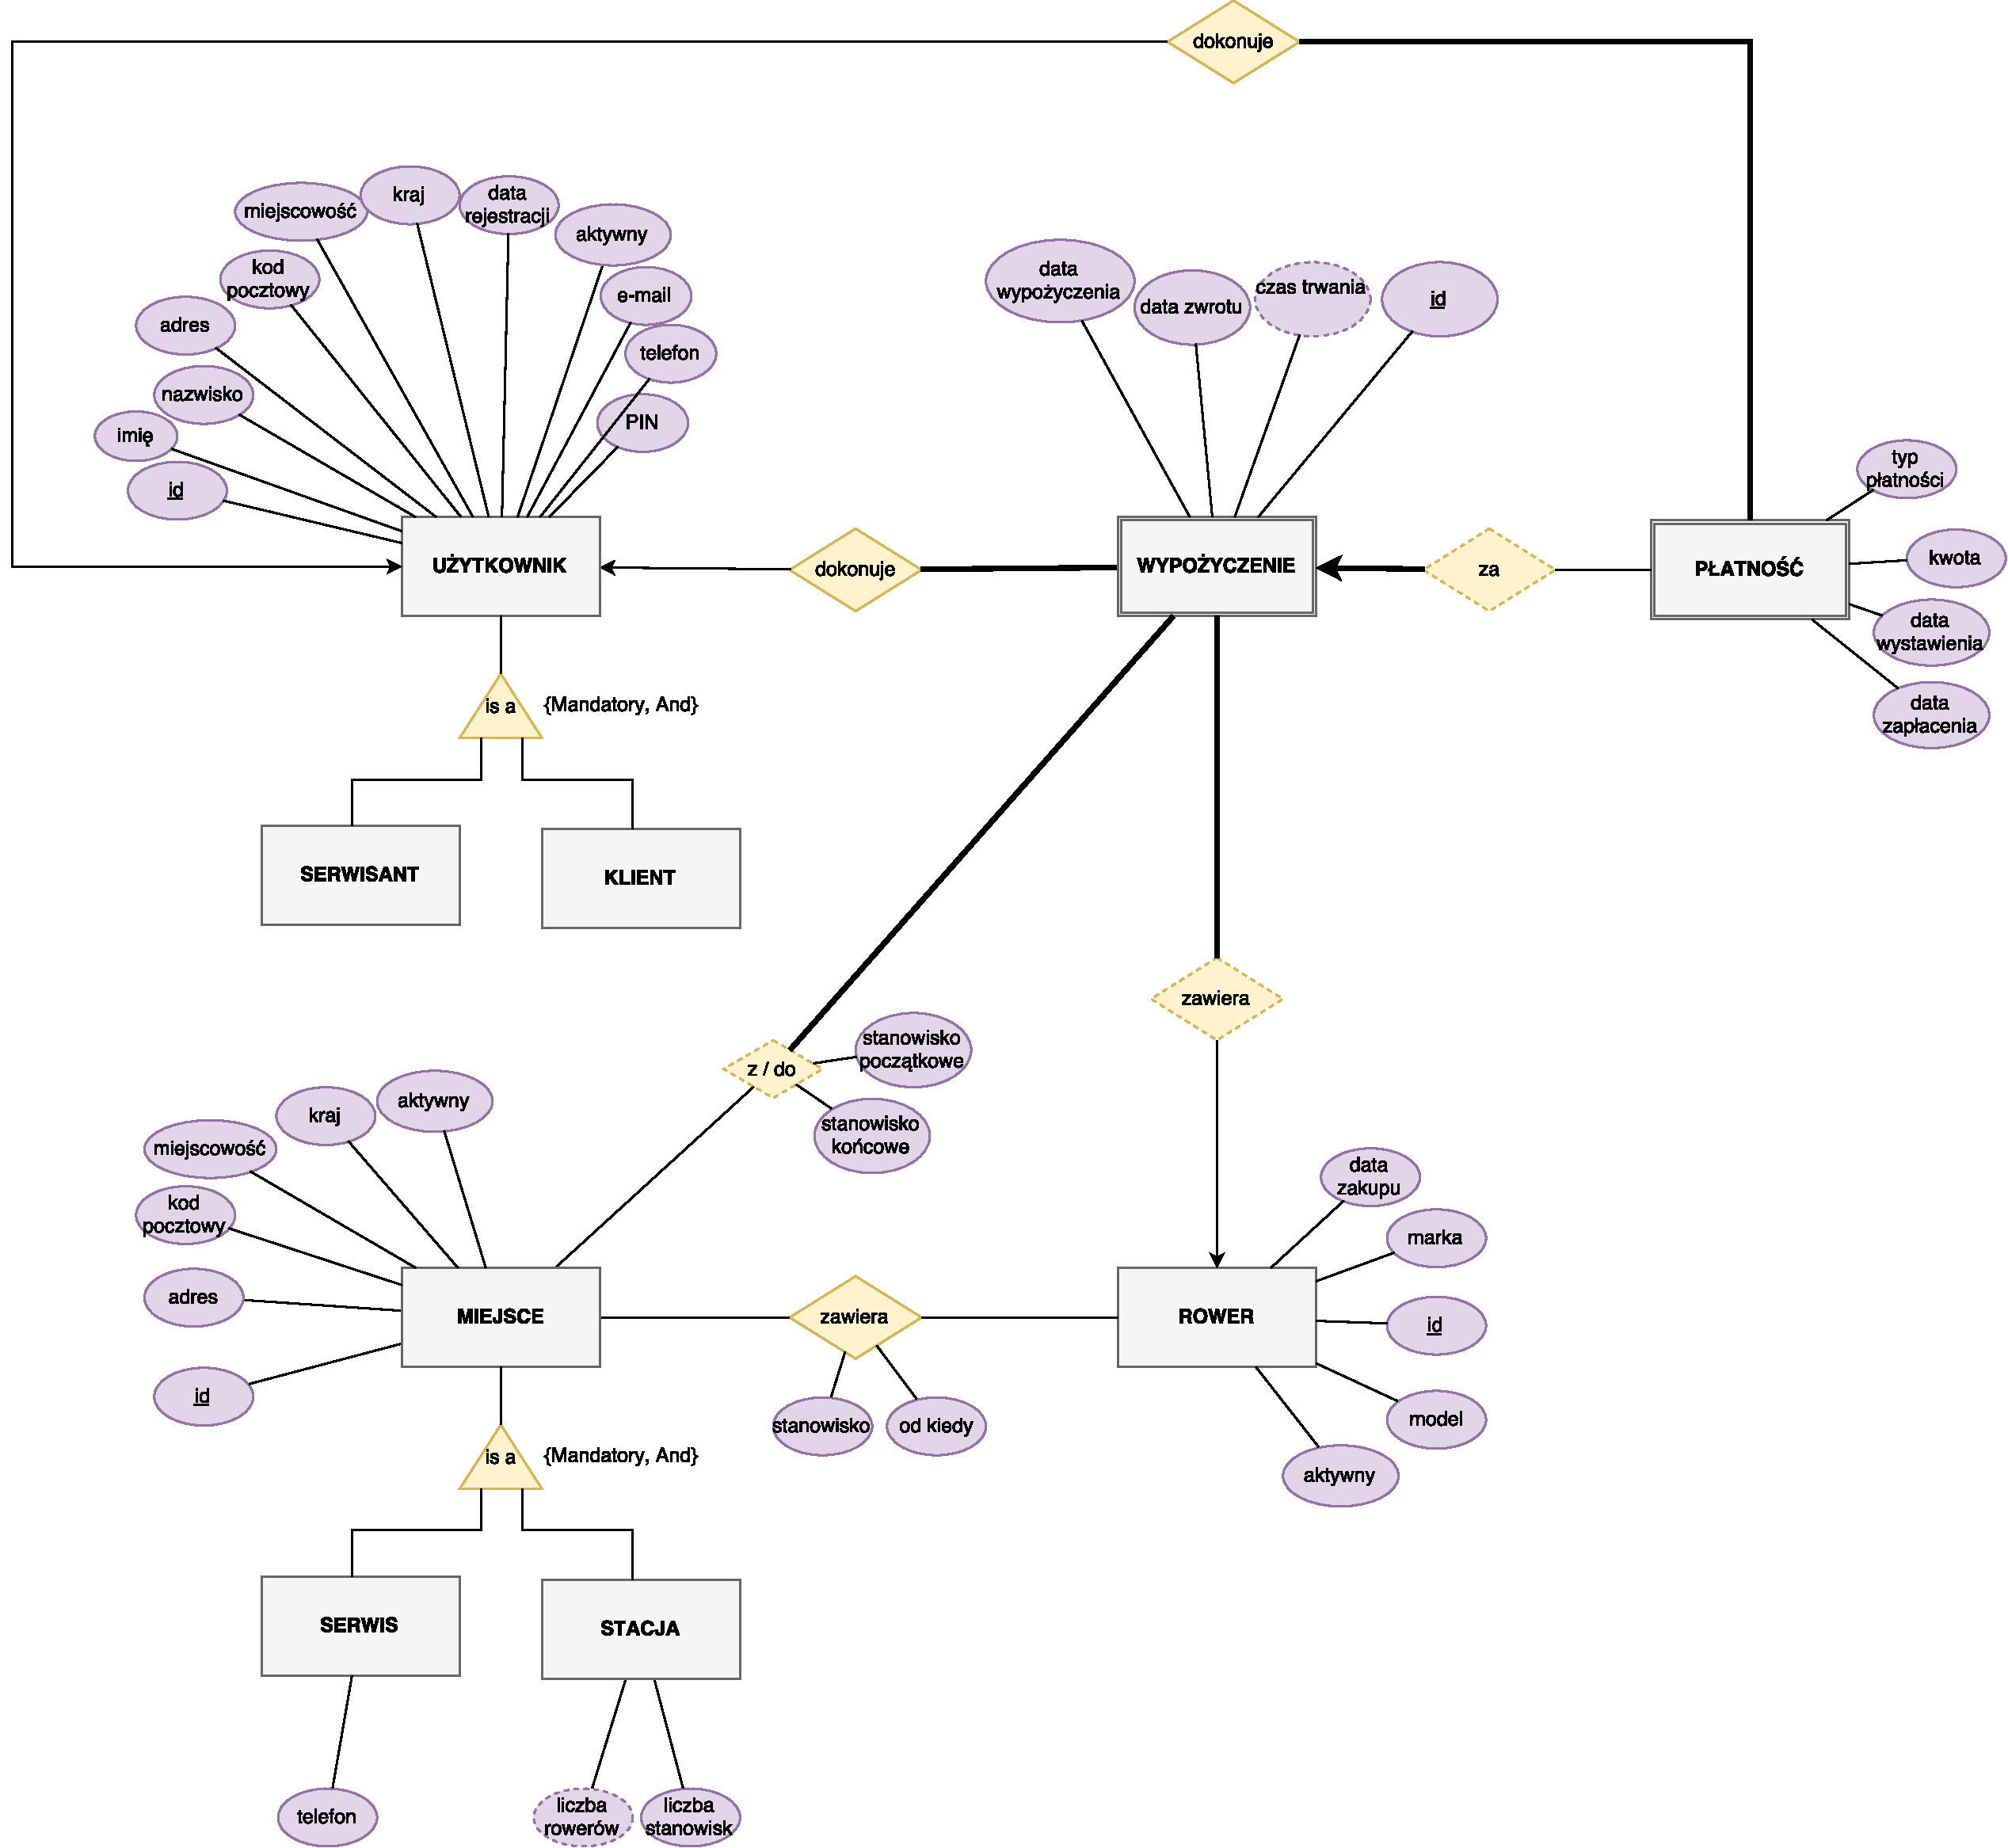
\includegraphics[width=\paperwidth, height=\paperheight, keepaspectratio]{conceptualmodel.pdf}}
\end{figure}

\subsection{Komentarz}
Na diagramie widnieje dziewięć encji.
Cztery z nich są oczywiste z punktu widzenia zagadnienia rowerów miejskich.
Mamy użytkowników, rowery, miejsca oraz wypożyczenia.
Użytkownicy mogą być jednym z dwóch typów: klientem lub serwisantem. Mimo że na diagramie użytkownik
ma atrybut PIN, to tak naprawdę nie będziemy tego hasła pamiętać. Więcej o tym pod koniec tej sekcji.
Tak samo miejsca mogą być jednym z dwóch typów: stacją lub serwisem.
Oczywiście stacje i serwisy mają swoje własne charakterystyczne cechy takie jak liczba stanowisk
na stacji bądź telefon do serwisu.
\newline
\newline
Użytkownicy dokonują wypożyczeń, które obejmują rowery (1 rower na wypożyczenie)
oraz 2 miejsca (początkowe i końcowe) a także stanowiska początkowe oraz końcowe.
Wypożyczenie obejmuje dwie sytuacje: wypożyczenie roweru przez klienta oraz przewiezienie roweru przez serwisanta.
Miejsca docelowe i końcowe mogą być albo serwisem albo stacją,
klient oczywiście będzie wypożyczał i zwracał rowery ze stacji, natomiast serwisant nie ma takiego ograniczenia.
Gdy jednym z miejsc wypożyczenia jest serwis,
to stanowisko nie ma wówczas żadnego znaczenia (W serwisach nie ma stanowisk z tego, co wiem).
\newline
\newline
Rowery znajdują się albo na stacjach, albo są wypożyczone, albo znajdują się w serwisie
(Na diagramie relacja Rower-Miejsce).
Za wypożyczenia naliczane są płatności, które zostały przedstawione jako kolejna encja.
Księgowy zajmujący się płatnościami może nakładać płatności
związane z trzema źródłami: wypożyczeniem, rejestracją, karą.
Wypożyczenie w płatności może być nullem, jeśli płatność dotyczy rejestracji.
\newline
\newline
\textbf{Uwaga:} W modelu fizycznym jest więcej tabel, widoków etc niż widać na tym diagramie.
Nie zostały one umieszczone, ponieważ nie są one ważne z punktu widzenia umodelowania zagadnienia rowerów miejskich.
Przykładem mógłby być sposób uwierzytelniania użytkowników. Loginem jest telefon, PIN jest hasłem, lecz w bazie danych
pamiętamy tak naprawdę losowy salt oraz hash skonkatenowanego salt'a z PINem podanym przez użytkownika.
\newline
\newline
Nieopisane więzy są całkiem oczywiste, nie znalazłem żadnych bardziej skomplikowanych więzów:
\begin{enumerate}
	\item Liczba stanowisk na stacji musi być nieujemna.
	\item Rower może być tylko na nieujemnym stanowisku (Na stacji).
	\item Stanowiska z których wypożyczono oraz do których zwrócono rowery muszą być albo NULL albo nieujemne.
	\item Czas zwrotu roweru musi być nie wcześniejsze niż czas wypożyczenia roweru.
	\item Kwota naliczona w płatności musi być nieujemna.
	\item Data pokrycia płatności musi być nie wcześniejsza niż data jej wystawienia.
\end{enumerate}

\subsection{Opis ról}
\subsubsection{Rola klienta}
\begin{enumerate}
	\item Może dodawać nowe wypożyczenia i aktualizować swoje wypożyczenie.
	\item Prawo do wglądu do historii wypożyczeń.
	\item Prawo do wglądu do historii płatności.
	\item Może zobaczyć, gdzie są stacje.
\end{enumerate}

\subsubsection{Rola serwisanta}
\begin{enumerate}
	\item Może przewozić rowery (Między stacjami i serwisami).
	\item Może sprawdzać, gdzie są rowery.
	\item Może sprawdzać, ile rowerów jest na której stacji.
	\item Może przeglądać katalog rowerów oraz dodawać nowe.
	\item Może przeglądać katalog stacji oraz serwisów oraz dodawać nowe.
\end{enumerate}

\subsubsection{Rola księgowego}
\begin{enumerate}
	\item Ma prawo do modyfikacji oraz odczytu danych płatności.
	\item Ma prawo do odczytu historii wypożyczeń.
	\item Ma prawo do odczytu danych użytkowników i aktywowania/dezaktywowania użytkowników.
	\item Nakłada płatności na użytkowników.
	\item Znajduje wypożyczenia z brakiem zwrotu roweru i nakłada kary na użytkowników wypożyczających.
\end{enumerate}

\section{Instalacja aplikacji}
Docelowo instalacja aplikacji jest przeznaczona na linuxy, konkretnie opisana zostanie procedura instalacji na Ubuntu.
W przypadku dystrybucji nie będących pochodną Ubuntu proces instalacji zależności może wyglądać inaczej.
\subsection{Wymagania}
Do instalacji aplikacji potrzebne są następujące zależności:
\begin{enumerate}
	\item openjdk-7-jdk
	\item postgresql - przynajmniej wersja 9.3 (Najlepiej wersja 9.4)
	\item postgresql-contrib (Zawiera moduł pgcrypto używany przy uwierzytelnianiu)
	\item maven2 (Manager zależności projektu)
	\item tomcat8 albo tomcat7 (Serwer)
\end{enumerate}

\subsection{Instalacja oraz uruchamianie}
Poniższe polecenia uruchamiamy znajdując się w katalogu projektu ("/project"). Jeśli zainstalowano
tomcat7, to tomcat8 należy zmienić na tomcat7.
\begin{lstlisting}[language=bash]
	$ sudo -u postgres psql -f src/main/resources/physicalmodel.sql
	$ mvn package
	# cp target/project.war /var/lib/tomcat8/webapps/
	# service tomcat8 start
\end{lstlisting}
\textbf{Wyjaśnienie:} Pierwsza z komend tworzy bazę danych z podanego modelu fizycznego. Operacja ta wymaga
zalogowania się w postgresie na konto superużytkownika, domyślnym superużytkownikiem jest ,,postgres".
W przypadku, gdy nie ma takiego superużytkownika, należy zalogować się na jakiegoś innego superużytkownika.

Drugie polecenia uruchamia maven, który pobiera zależności opisane w pliku pom.xml i buduje plik project.war.

Następnie wyprodukowany project.war kopiujemy do katalogu, w ktorym serwer tomcat przechowuje aplikacje webowe.

Na samym końcu uruchamiamy serwer. Aby połączyć się z projektem należy użyć przeglądarki
internetowej i połączyć się z adresem \emph{localhost:8080/project}.

\section{Dokumentacja aplikacji}
\subsection{Technologia}
Aplikacja jest oczywiście webowa. Została napisana w Javie z wykorzystaniem frameworków Spring MVC oraz
Hibernate ORM. Wykorzystano właściwości mapowania obiektowo relacyjnego takie jak: leniwe wczytywanie, cache pierwszego poziomu,
filtry, oraz dziedziczenie encji (Np. Hibernate pozwala nam utrzymywać klasę Miejsce
oraz jej podział na podklasy - Stacja i Serwis według wartości kolumny ,,rodzaj'' w tabeli miejsce).

\subsection{Struktura projektu}
Pliki w katalogu src/main/java zostały podzielone na paczki (ang. packages) odpowiednio według kategori:
\begin{enumerate}
	\item com.entities - Klasy reprezentujące encje na diagramie E-R implementowane za pomocą Hibernate.
	\item com.dao - Zastosowanie wzorca projektowego Data Access Object - w tej paczce znajdują się interfejsy i implementacje.
	\item com.controllers - Kontrolery do wzorca projektowego MVC oferowanego przez framework Spring. Odpowiedzialne za przetwarzanie żądań.
	\item com.services - Usługi, z których mogą korzystać kontrolery. Używają m.in. instancji klas DAO do wykonywania poleceń kontrolerów.
		W odróżnieniu od klas DAO, serwisy posiadają w sobie logikę, klasy DAO po prostu wydobywają dane z bazy danych.
	\item com.businessLogic - Pozostałe klasy używane przy przetwarzaniu żądań (Własne wyjątki, klasy wrappery na dane uzyskiwane z formularzy etc.).
\end{enumerate}

Oprócz tego w katalogu src/main/webapp/WEB-INF znajdują się pliki konfiguracyjne aplikacji oraz katalog z widokami (do wzorca MVC).

\subsection{Możliwości aplikacji}
Strona główna udostępnia dwie możliwości: logowanie oraz rejestrację.
\begin{figure}[p]
\centerline{
	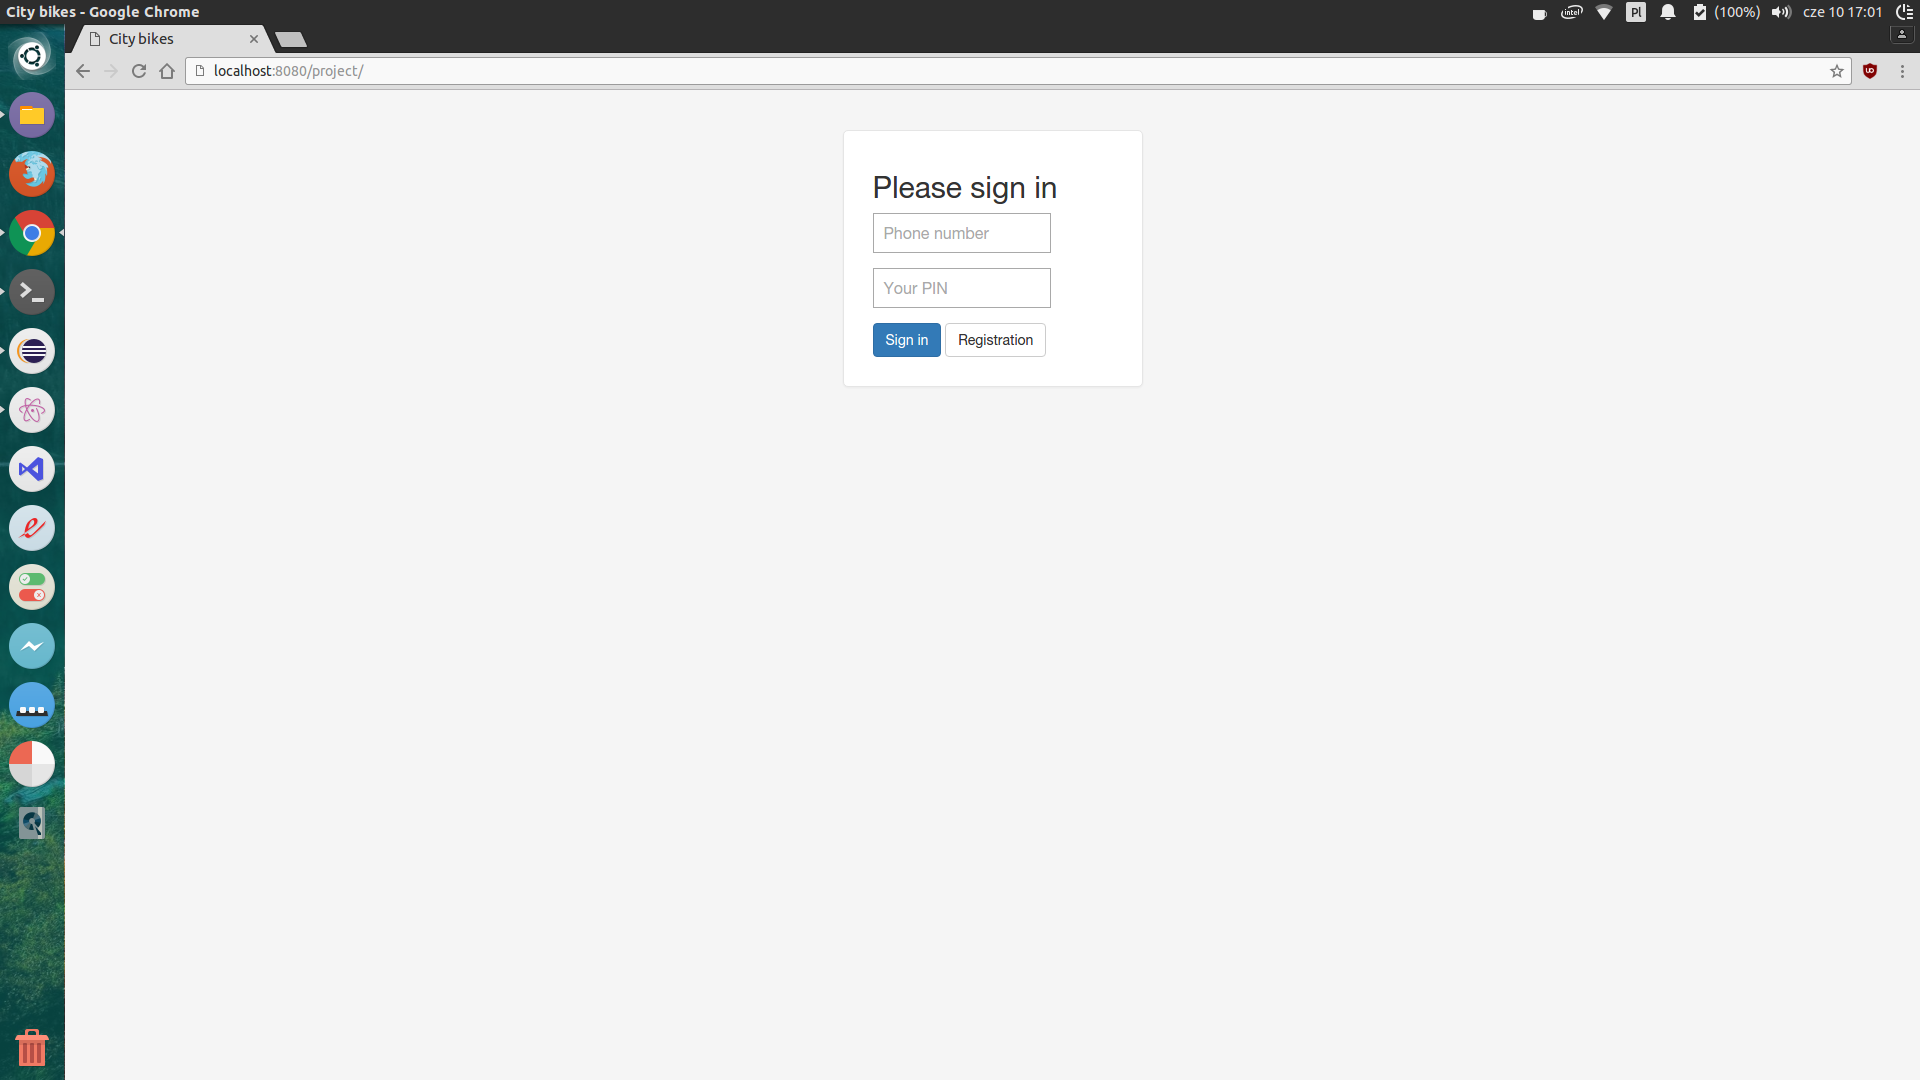
\includegraphics[width=\paperwidth, height=\paperheight, keepaspectratio]{screenshots/loginscreen.png}}
	\caption{Strona główna}
\end{figure}
\begin{figure}[p]
\centerline{
	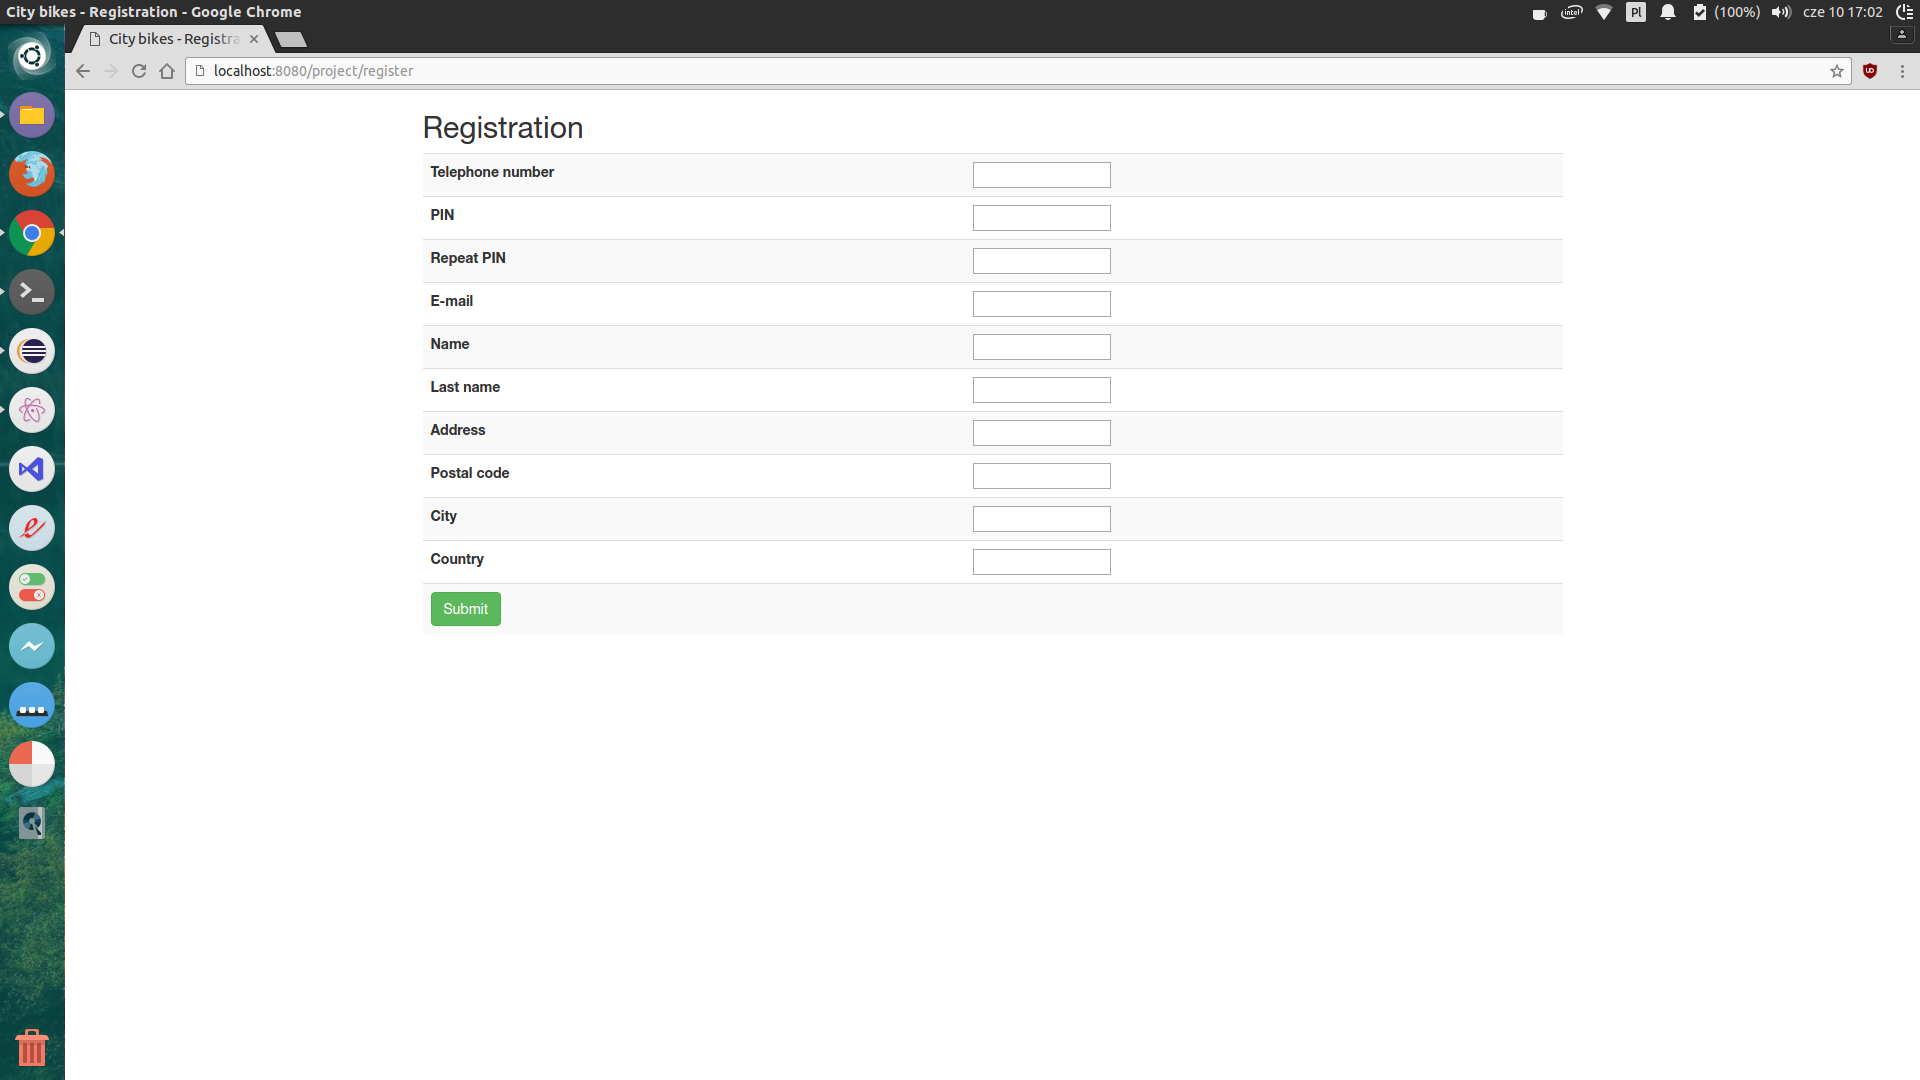
\includegraphics[width=\paperwidth, height=\paperheight, keepaspectratio]{screenshots/registration.png}}
	\caption{Rejestracja}
\end{figure}

\subsubsection{Użytkownik}
Po zalogowaniu użytkownika wita jego strona główna, na której wypisane są jego ostatnie wypożyczenia.
\begin{figure}[p]
\centerline{
	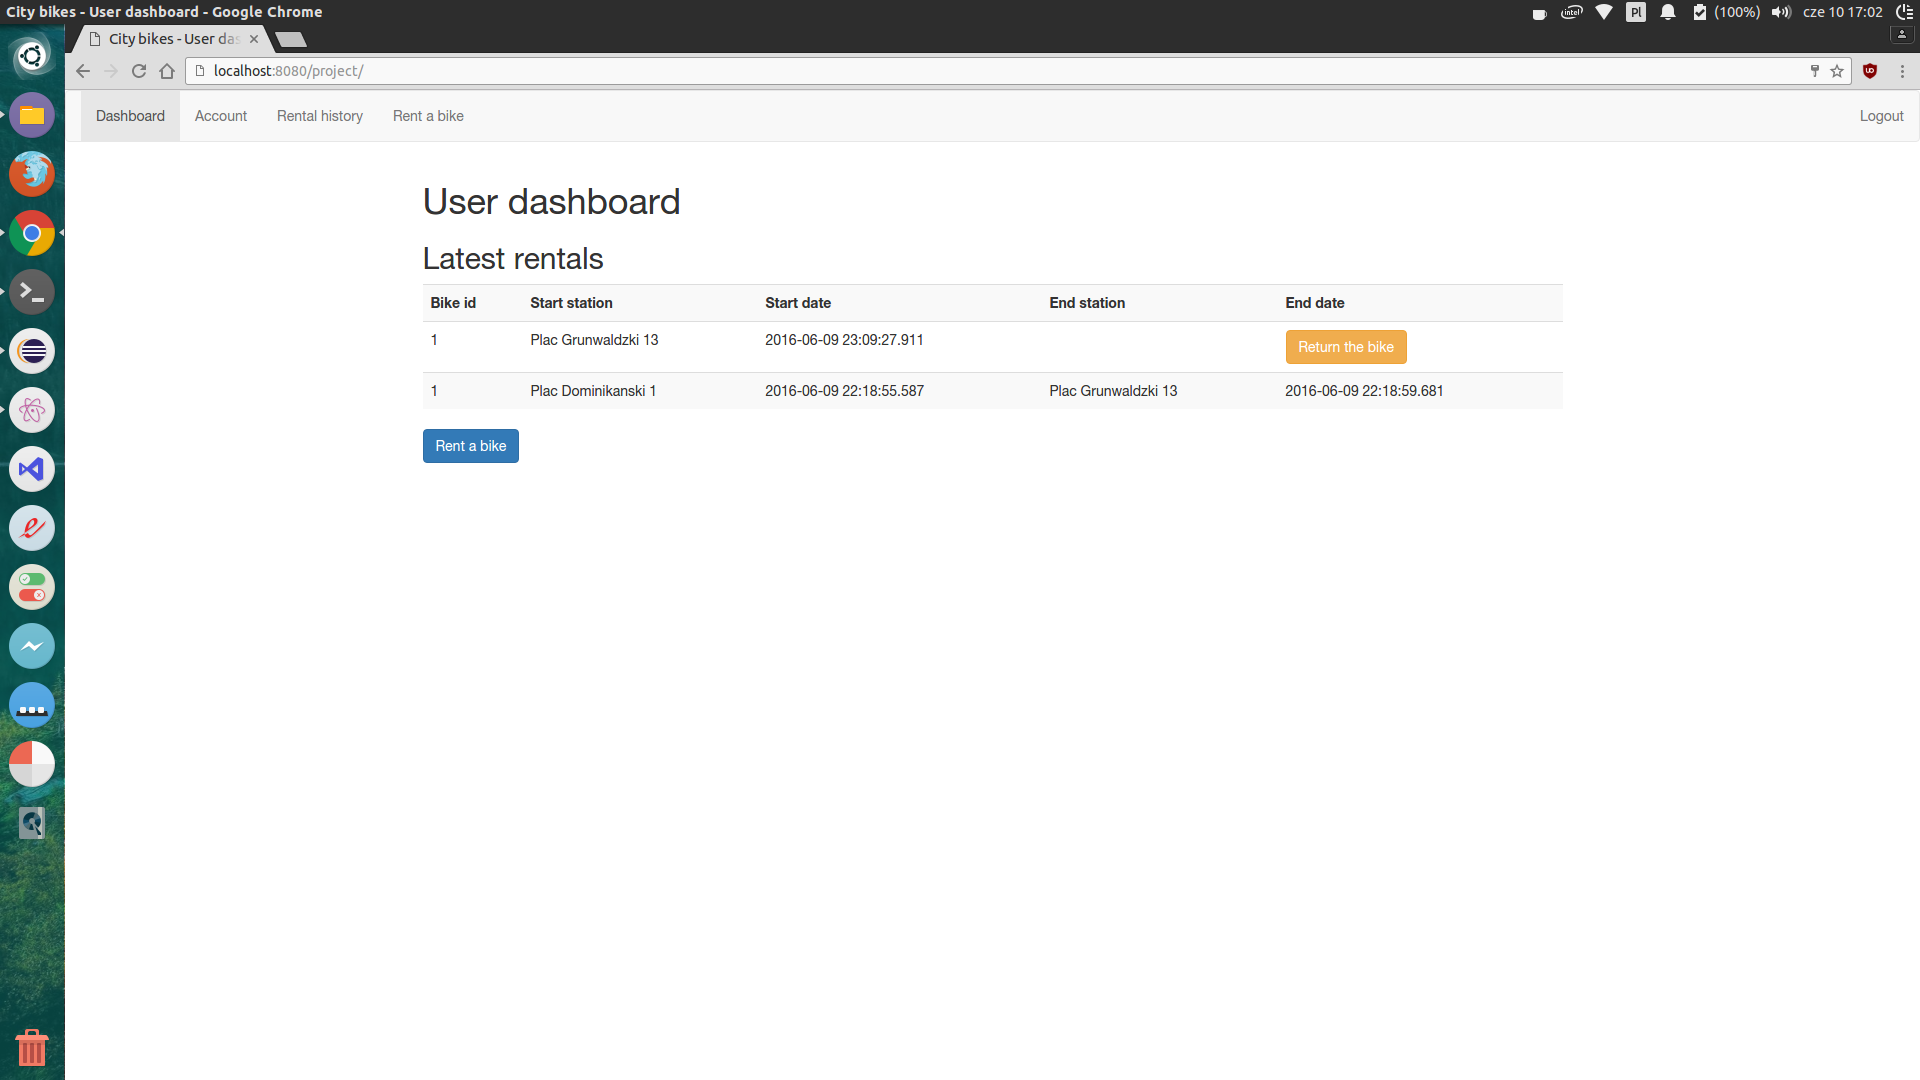
\includegraphics[width=\paperwidth, height=\paperheight, keepaspectratio]{screenshots/userdashboard.png}}
	\caption{Strona główna użytkownika}
\end{figure}
Na stronie głównej użytkownik ma następujące możliwości:
\begin{enumerate}
	\item Przeglądnięcie swojego konta + zmiana informacji osobowych.
	\item Przeglądnięcie historii wypożyczeń oraz płatności.
	\item Wypożyczenie roweru.
	\item Wylogowanie się.
\end{enumerate}

\begin{figure}[p]
\centerline{
	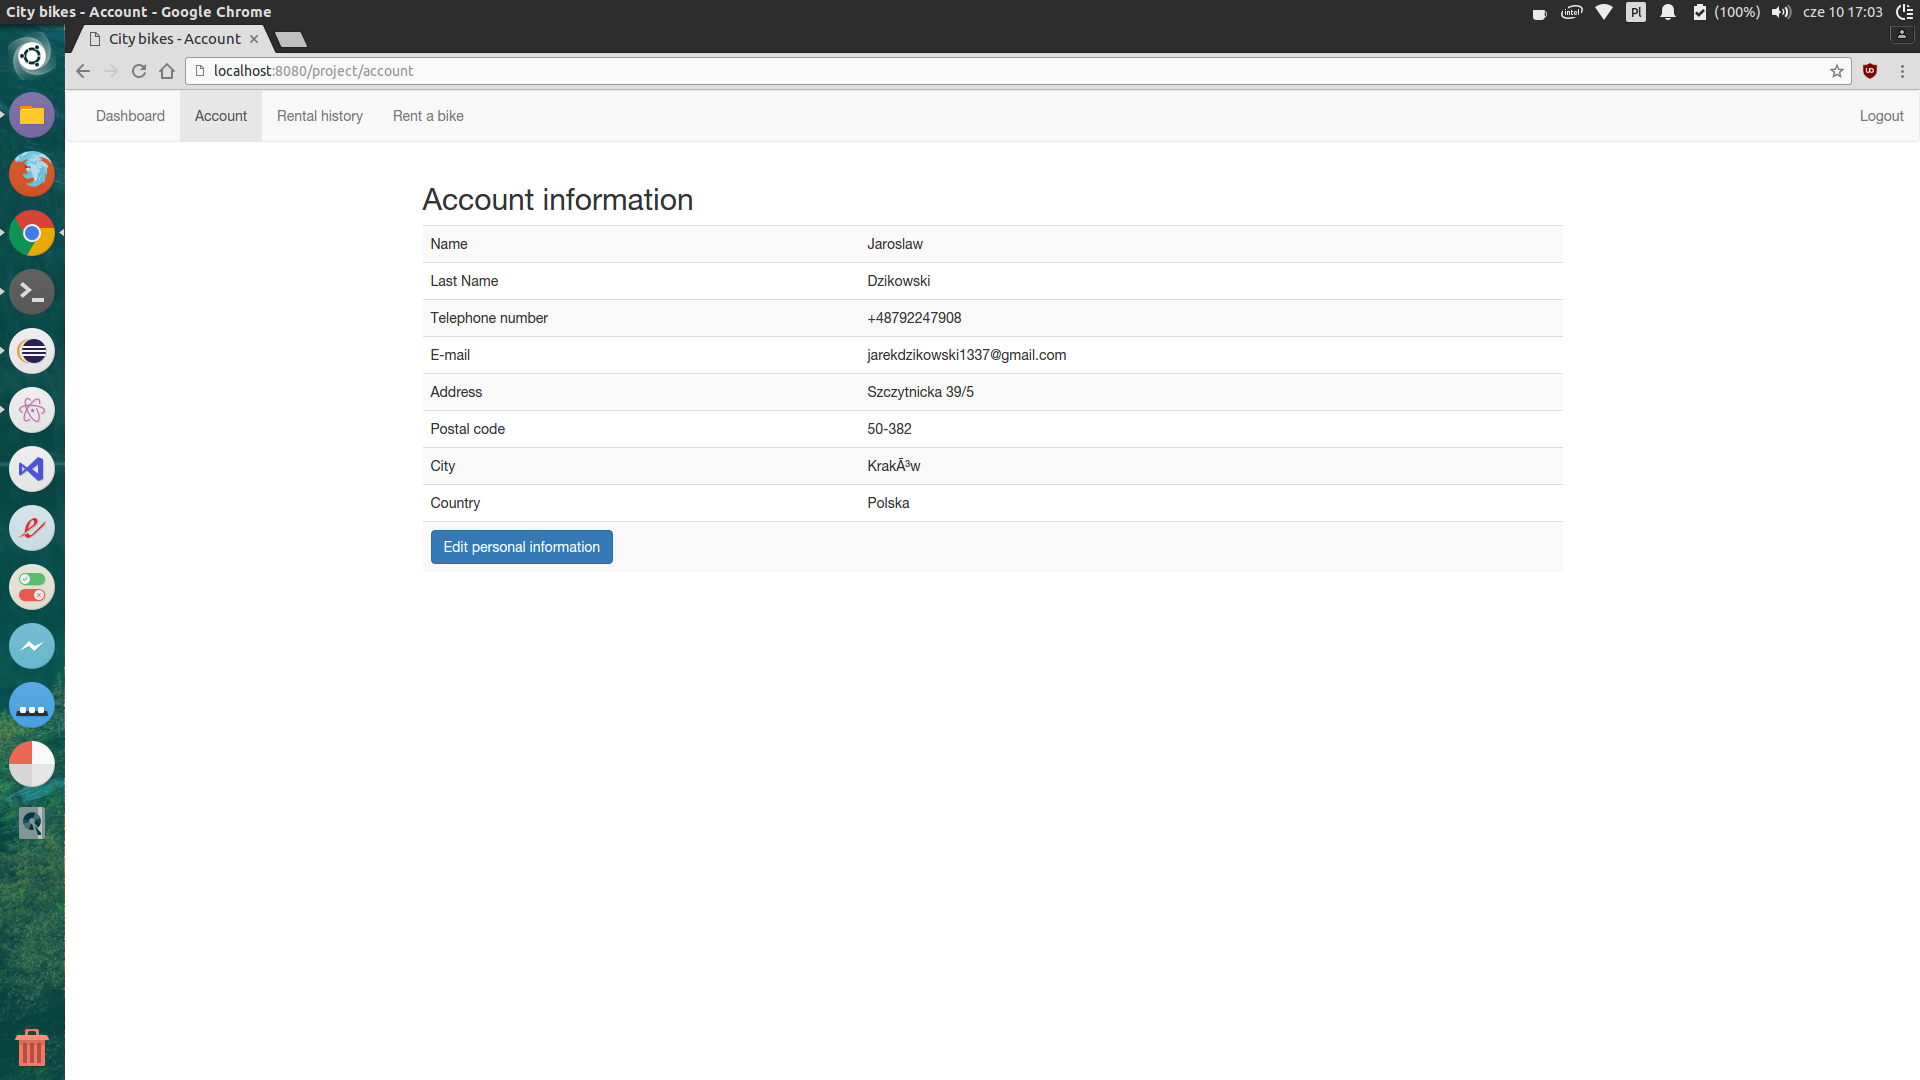
\includegraphics[width=\paperwidth, height=\paperheight, keepaspectratio]{screenshots/account.png}}
	\caption{Konto użytkownika}
\end{figure}
\begin{figure}[p]
\centerline{
	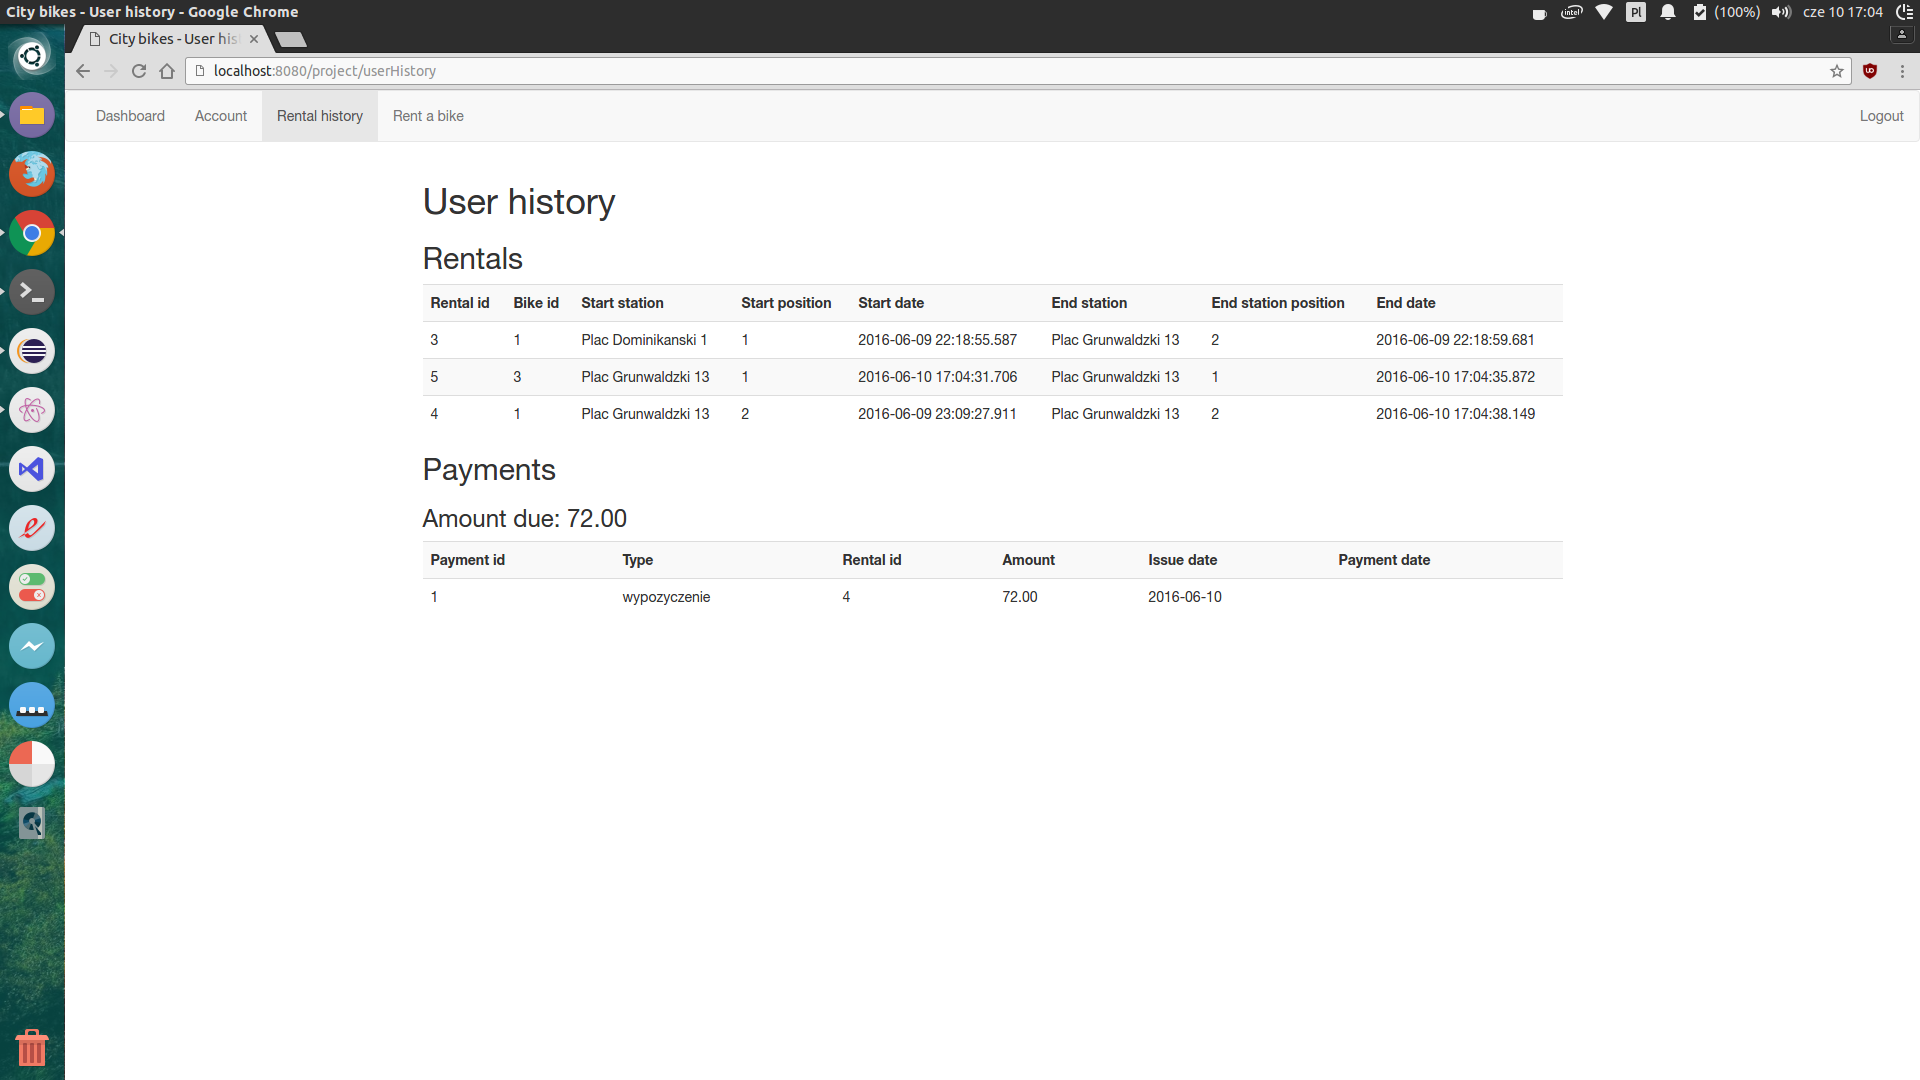
\includegraphics[width=\paperwidth, height=\paperheight, keepaspectratio]{screenshots/userHistory.png}}
	\caption{Historia użytkownika}
\end{figure}
\begin{figure}[p]
\centerline{
	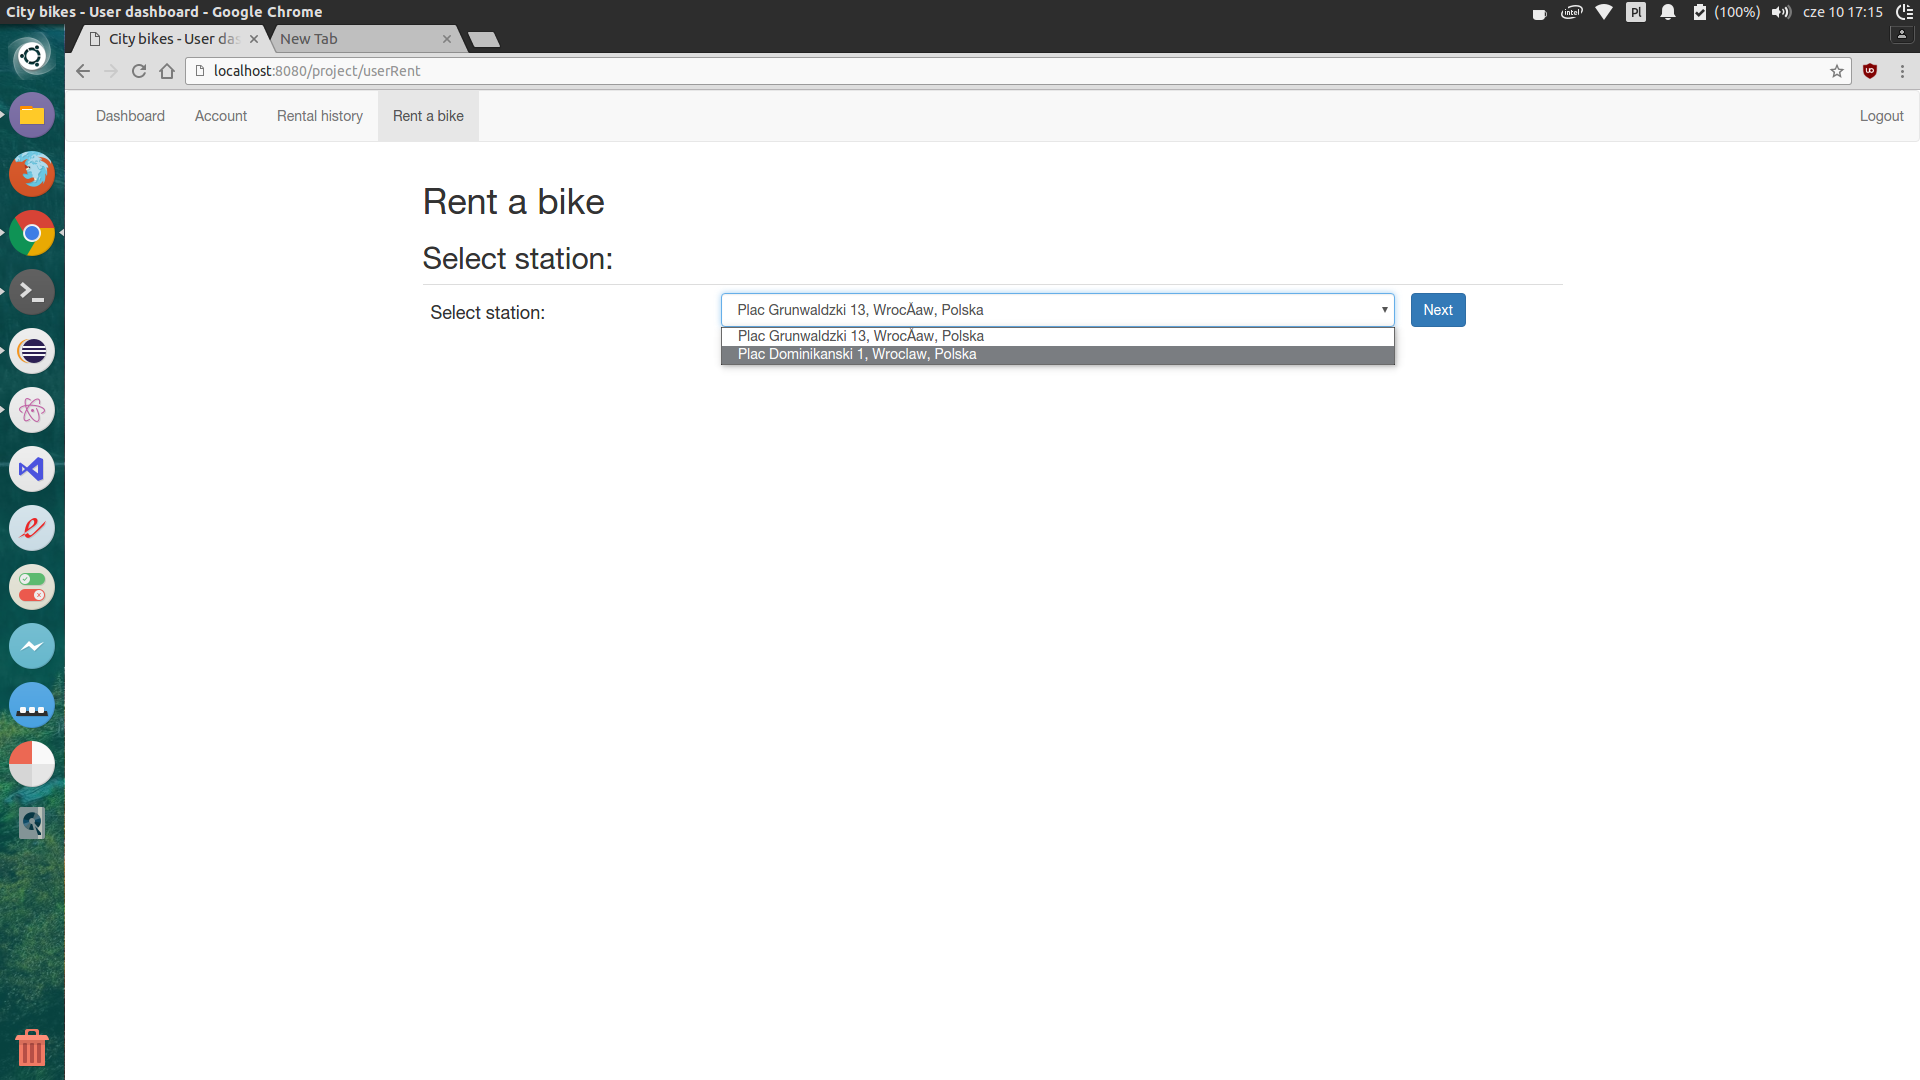
\includegraphics[width=\paperwidth, height=\paperheight, keepaspectratio]{screenshots/rentbike.png}}
	\caption{Wypożyczenie roweru}
\end{figure}

\subsection{Administrator}
Administrator ma więcej możliwości. Po zalogowaniu się widzi swoją stronę główną,
gdzie może zobaczyć swoje aktywne przeniesienia rowerów oraz ma do wyboru ma następujące akcje:
\begin{enumerate}
	\item Przejście do strony zarządzania użytkownikami (Zmiana typu [klient/serwisant], usuwanie).
	\item Przejście do strony zarządzania rowerami (Dodawanie, edytowanie, usuwanie).
	\item Przejście do strony zarządzania miejscami (Dodawanie, edytowanie, usuwanie).
	\item Przejście do strony ze wszystkimi aktywnymi wypożyczeniami.
	\item Wypożyczenie (Przeniesienie) roweru.
	\item Wylogowanie.
\end{enumerate}
\begin{figure}[p]
\centerline{
	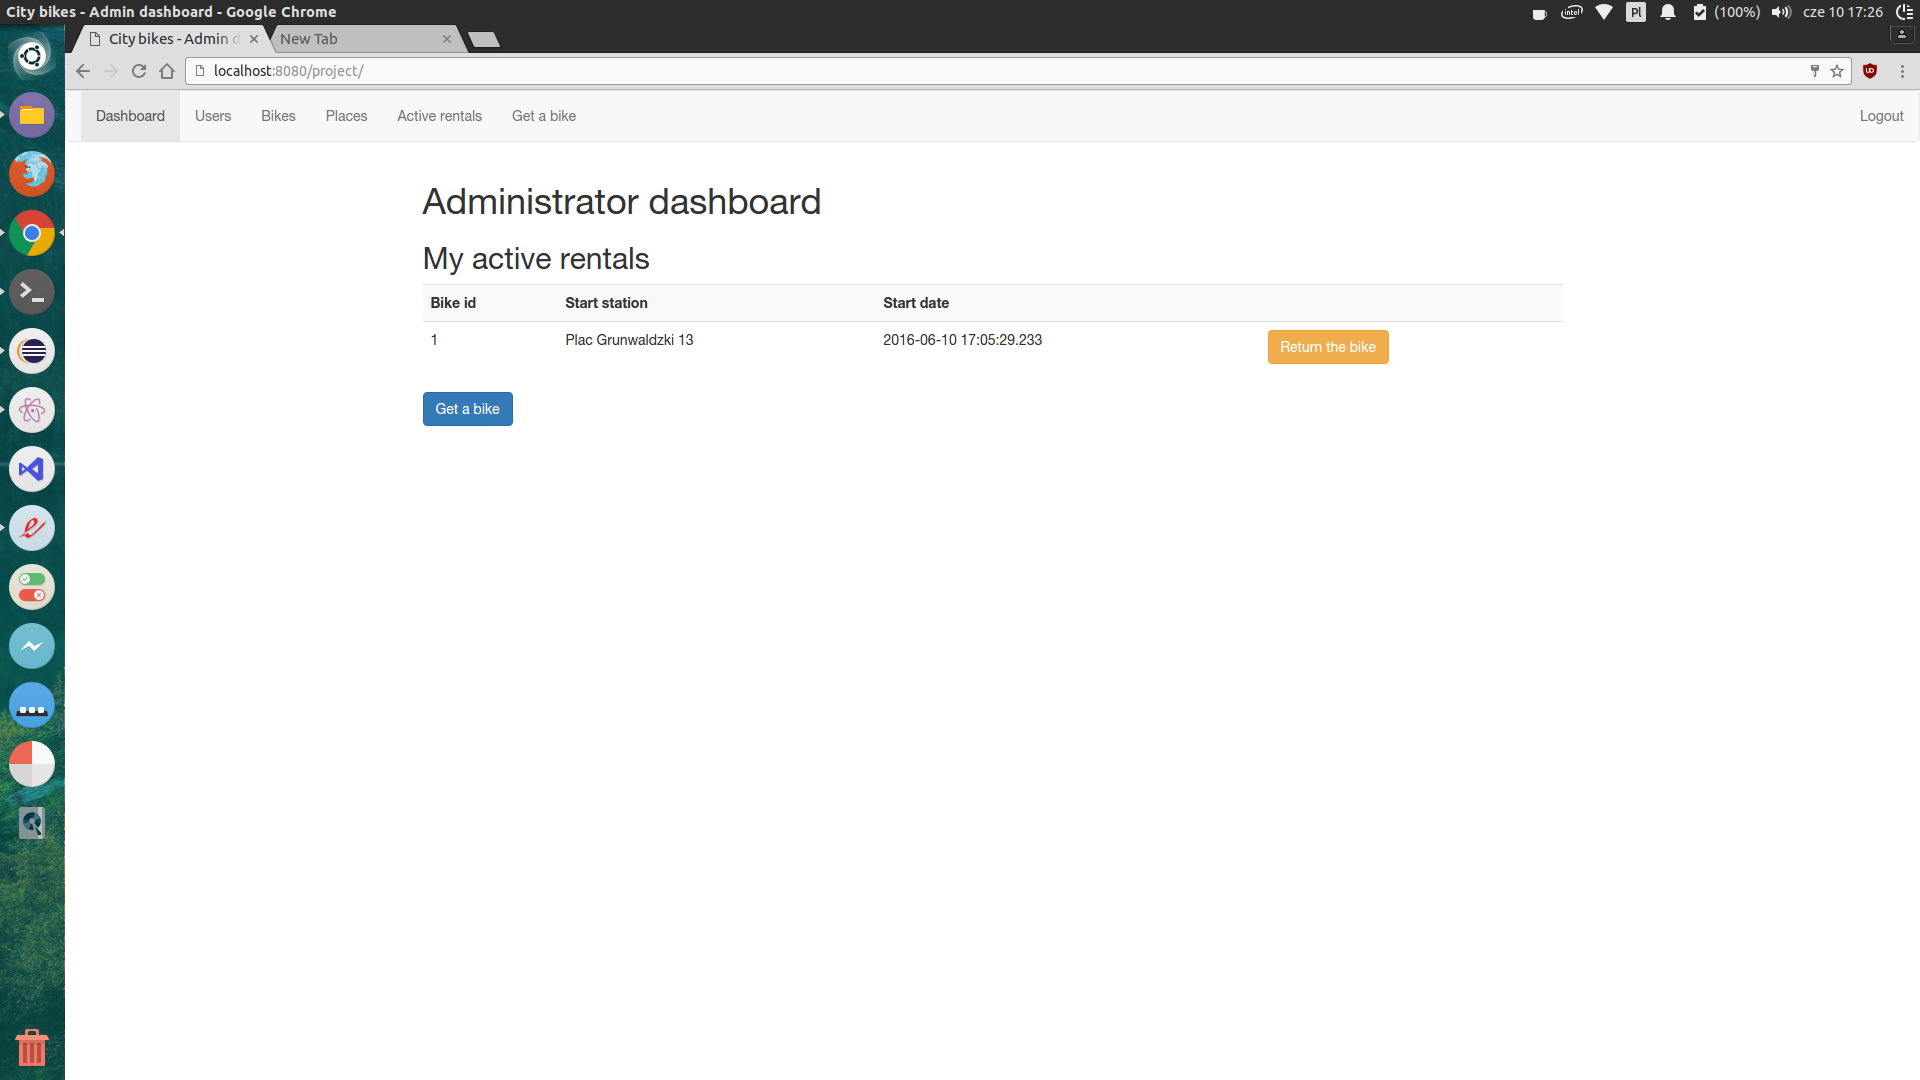
\includegraphics[width=\paperwidth, height=\paperheight, keepaspectratio]{screenshots/admindashboard.png}}
	\caption{Strona główna administratora}
\end{figure}
\begin{figure}[p]
\centerline{
	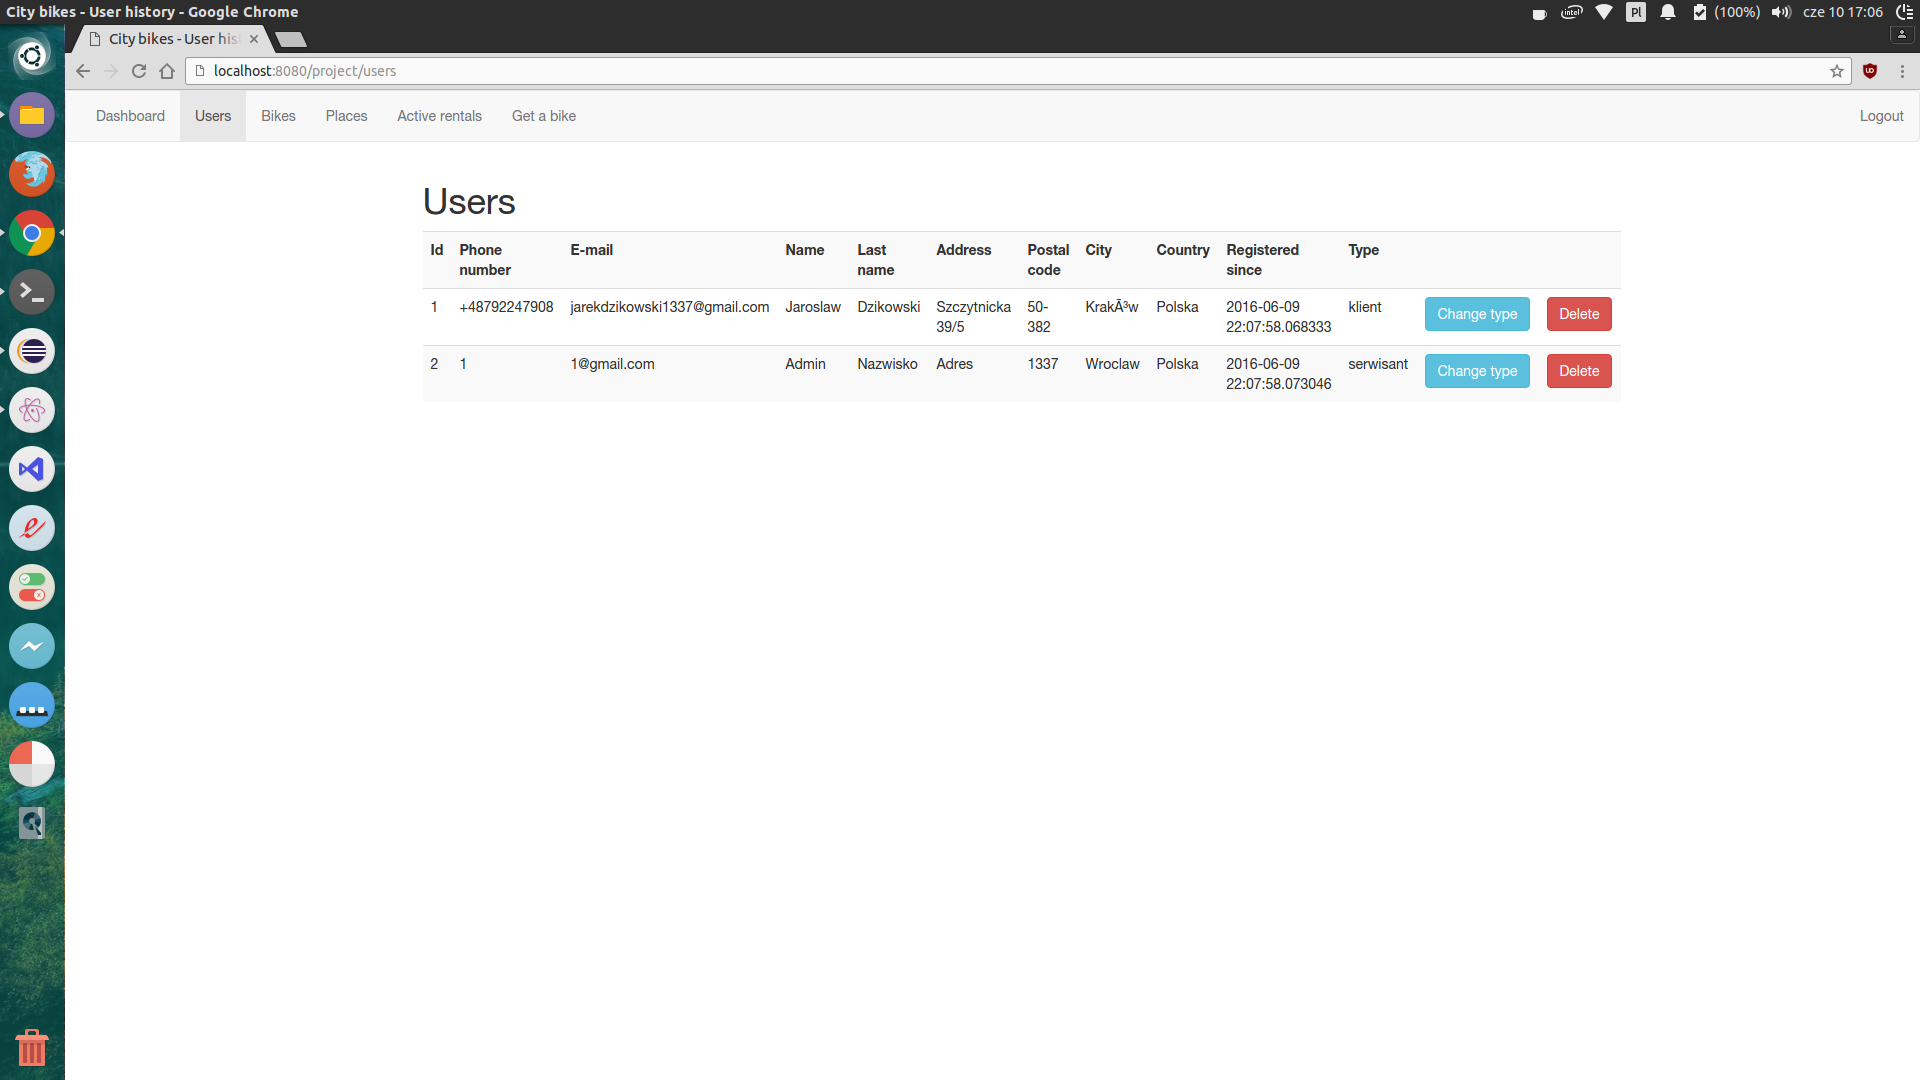
\includegraphics[width=\paperwidth, height=\paperheight, keepaspectratio]{screenshots/adminusers.png}}
	\caption{Zarządzanie użytkownikami}
\end{figure}
\begin{figure}[p]
\centerline{
	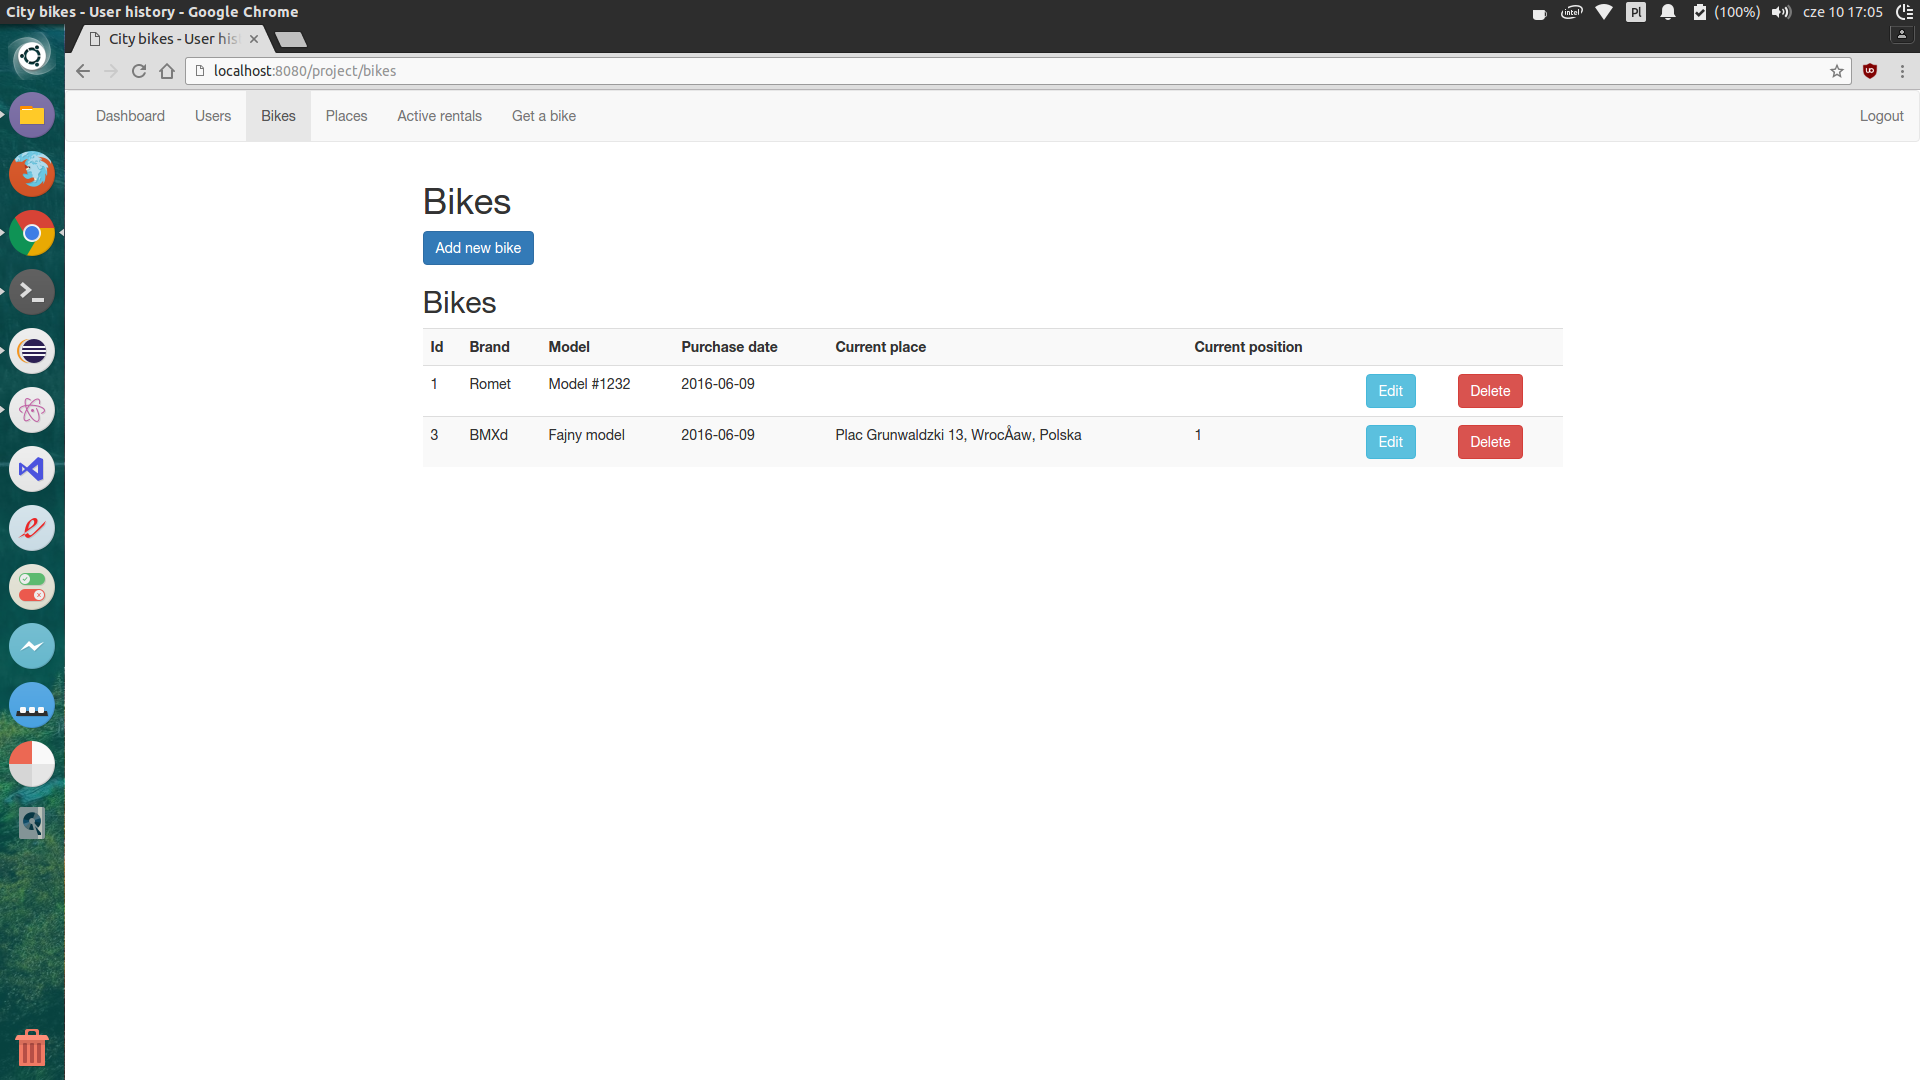
\includegraphics[width=\paperwidth, height=\paperheight, keepaspectratio]{screenshots/adminbikes.png}}
	\caption{Zarządzanie rowerami}
\end{figure}
\begin{figure}[p]
\centerline{
	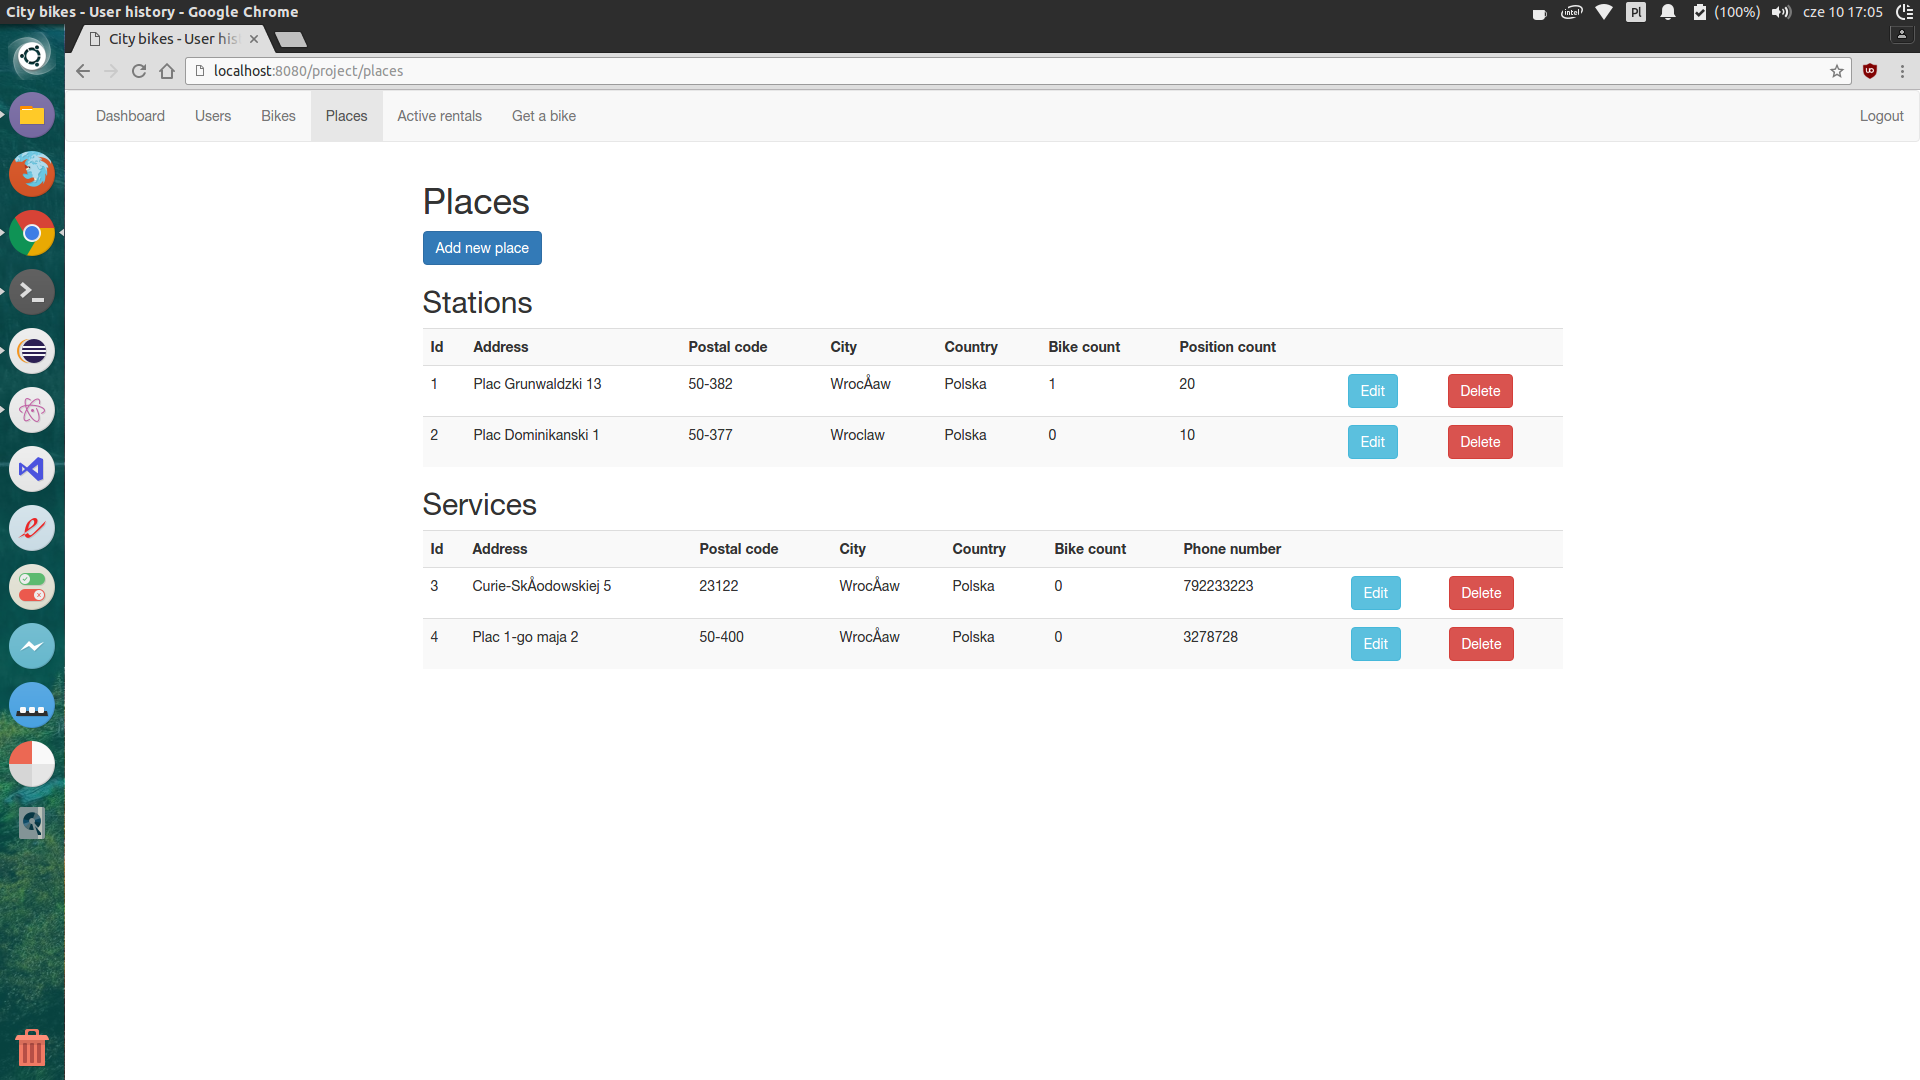
\includegraphics[width=\paperwidth, height=\paperheight, keepaspectratio]{screenshots/adminplaces.png}}
	\caption{Zarządzanie miejscami}
\end{figure}
\begin{figure}[p]
\centerline{
	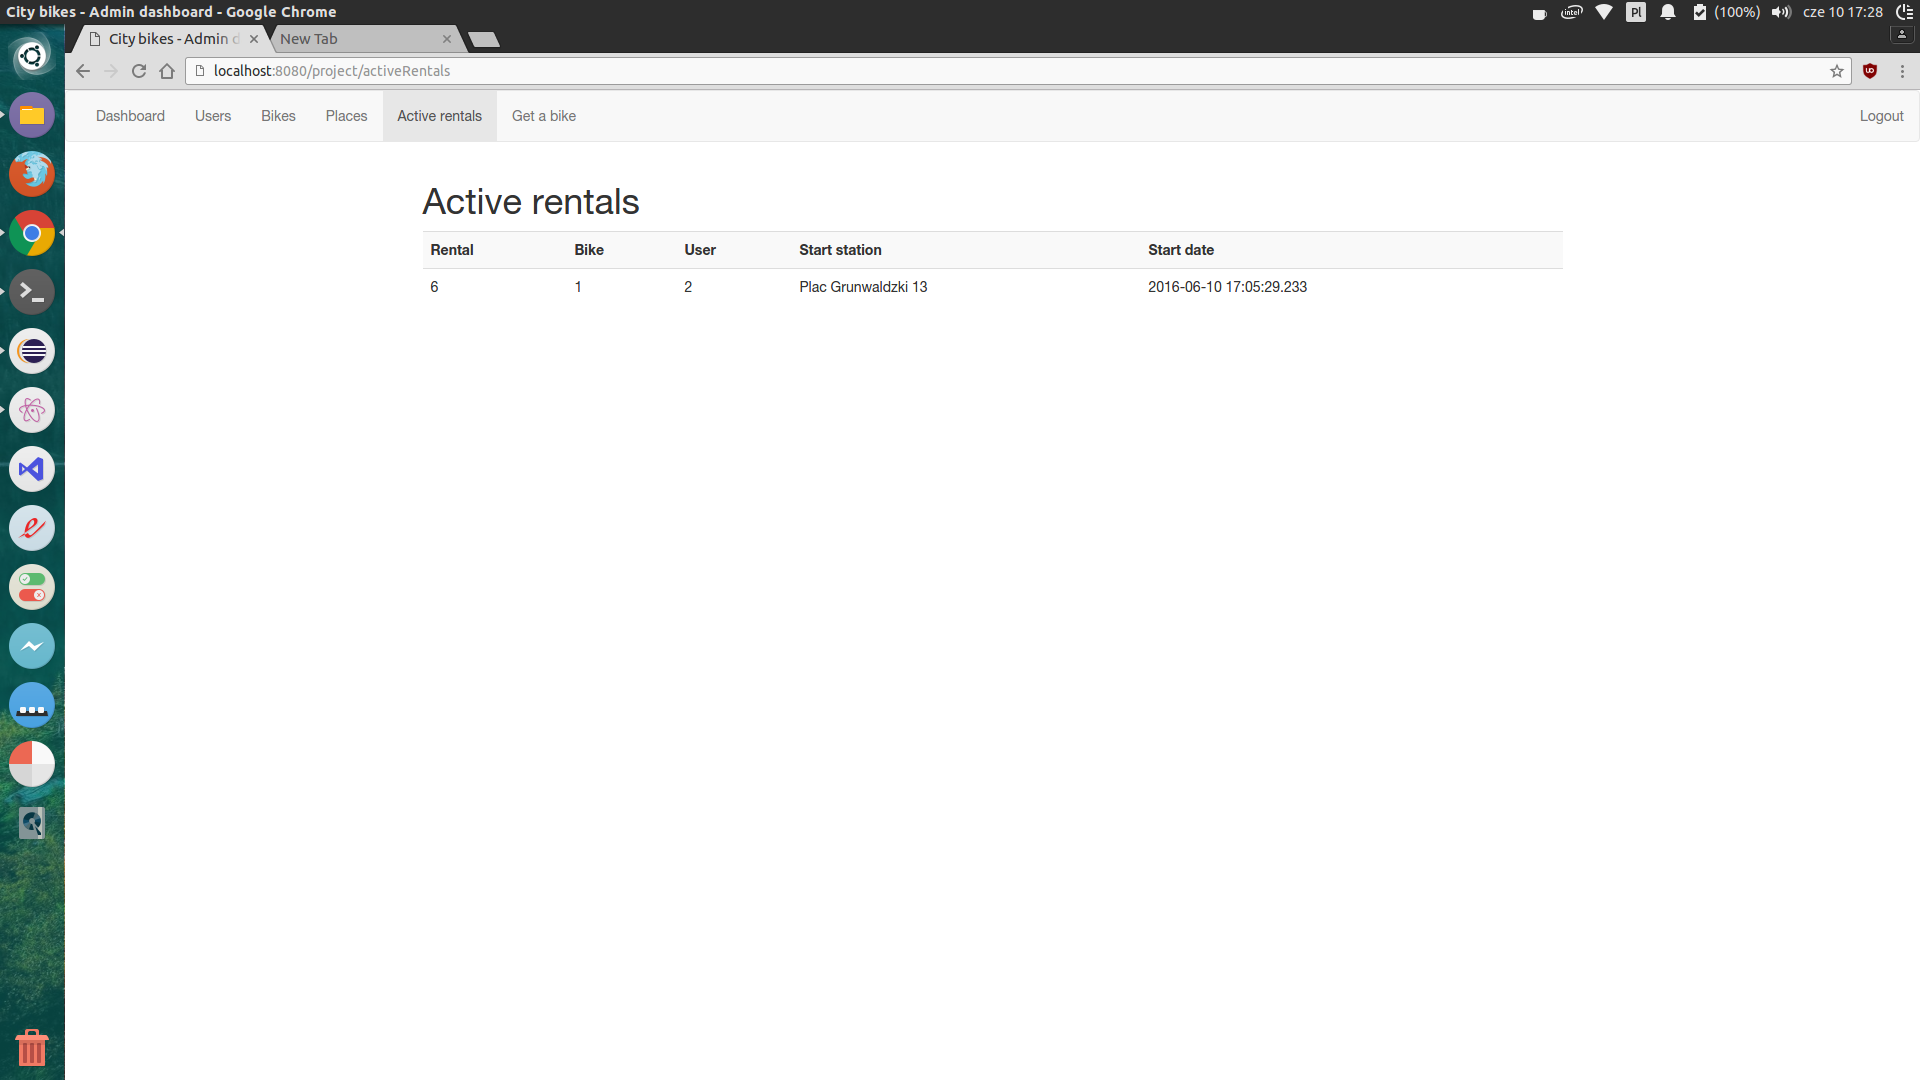
\includegraphics[width=\paperwidth, height=\paperheight, keepaspectratio]{screenshots/adminrentals.png}}
	\caption{Aktywne wypożyczenia}
\end{figure}

\end{document}
